\def\year{2019}\relax
%File: formatting-instruction.tex
\documentclass[letterpaper]{article} % DO NOT CHANGE THIS
\usepackage{aaai19}  % DO NOT CHANGE THIS
\usepackage{times}  % DO NOT CHANGE THIS
\usepackage{helvet} % DO NOT CHANGE THIS
\usepackage{courier}  % DO NOT CHANGE THIS
\usepackage[hyphens]{url}  % DO NOT CHANGE THIS
\usepackage{graphicx} % DO NOT CHANGE THIS
\urlstyle{rm} % DO NOT CHANGE THIS
\def\UrlFont{\rm}  % DO NOT CHANGE THIS
\usepackage{graphicx}  % DO NOT CHANGE THIS
\frenchspacing  % DO NOT CHANGE THIS
\setlength{\pdfpagewidth}{8.5in}  % DO NOT CHANGE THIS
\setlength{\pdfpageheight}{11in}  % DO NOT CHANGE THIS

\usepackage[utf8]{inputenc} % allow utf-8 input
\usepackage[UTF8]{ctex}
\usepackage{natbib}
\usepackage{amsmath}
\usepackage{mathtools}
\usepackage{subfigure} 
\usepackage{algorithm}
\usepackage{algorithmicx}
%PDF Info Is REQUIRED.
% For /Author, add all authors within the parentheses, separated by commas. No accents or commands.
% For /Title, add Title in Mixed Case. No accents or commands. Retain the parentheses.
 \pdfinfo{
/Title (AAAI Press Formatting Instructions for Authors Using LaTeX -- A Guide)
/Author (AAAI Press Staff, Pater Patel Schneider, Sunil Issar, J. Scott Penberthy, George Ferguson, Hans Guesgen)
} %Leave this	
% /Title ()
% Put your actual complete title (no codes, scripts, shortcuts, or LaTeX commands) within the parentheses in mixed case
% Leave the space between \Title and the beginning parenthesis alone
% /Author ()
% Put your actual complete list of authors (no codes, scripts, shortcuts, or LaTeX commands) within the parentheses in mixed case. 
% Each author should be only by a comma. If the name contains accents, remove them. If there are any LaTeX commands, 
% remove them. 

% DISALLOWED PACKAGES
% \usepackage{authblk} -- This package is specifically forbidden
% \usepackage{balance} -- This package is specifically forbidden
% \usepackage{caption} -- This package is specifically forbidden
% \usepackage{color (if used in text)
% \usepackage{CJK} -- This package is specifically forbidden
% \usepackage{float} -- This package is specifically forbidden
% \usepackage{flushend} -- This package is specifically forbidden
% \usepackage{fontenc} -- This package is specifically forbidden
% \usepackage{fullpage} -- This package is specifically forbidden
% \usepackage{geometry} -- This package is specifically forbidden
% \usepackage{grffile} -- This package is specifically forbidden
% \usepackage{hyperref} -- This package is specifically forbidden
% \usepackage{navigator} -- This package is specifically forbidden
% (or any other package that embeds links such as navigator or hyperref)
% \indentfirst} -- This package is specifically forbidden
% \layout} -- This package is specifically forbidden
% \multicol} -- This package is specifically forbidden
% \nameref} -- This package is specifically forbidden
% \natbib} -- This package is specifically forbidden -- use the following workaround:
% \usepackage{savetrees} -- This package is specifically forbidden
% \usepackage{setspace} -- This package is specifically forbidden
% \usepackage{stfloats} -- This package is specifically forbidden
% \usepackage{tabu} -- This package is specifically forbidden
% \usepackage{titlesec} -- This package is specifically forbidden
% \usepackage{tocbibind} -- This package is specifically forbidden
% \usepackage{ulem} -- This package is specifically forbidden
% \usepackage{wrapfig} -- This package is specifically forbidden
% DISALLOWED COMMANDS
% \nocopyright -- Your paper will not be published if you use this command
% \addtolength -- This command may not be used
% \balance -- This command may not be used
% \baselinestretch -- Your paper will not be published if you use this command
% \clearpage -- No page breaks of any kind may be used for the final version of your paper
% \columnsep -- This command may not be used
% \newpage -- No page breaks of any kind may be used for the final version of your paper
% \pagebreak -- No page breaks of any kind may be used for the final version of your paperr
% \pagestyle -- This command may not be used
% \tiny -- This is not an acceptable font size.
% \vspace{- -- No negative value may be used in proximity of a caption, figure, table, section, subsection, subsubsection, or reference
% \vskip{- -- No negative value may be used to alter spacing above or below a caption, figure, table, section, subsection, subsubsection, or reference

\setcounter{secnumdepth}{2} %May be changed to 1 or 2 if section numbers are desired.

% The file aaai19.sty is the style file for AAAI Press 
% proceedings, working notes, and technical reports.
%
\setlength\titlebox{2.5in} % If your paper contains an overfull \vbox too high warning at the beginning of the document, use this
% command to correct it. You may not alter the value below 2.5 in
\title{基于条件生成对抗网络的配准多模态脑MRI合成}
%Your title must be in mixed case, not sentence case. 
% That means all verbs (including short verbs like be, is, using,and go), 
% nouns, adverbs, adjectives should be capitalized, including both words in hyphenated terms, while
% articles, conjunctions, and prepositions are lower case unless they
% directly follow a colon or long dash
\author{\Large \textbf{Yili Qu,Wanqi Su,Chufu Deng,}\\ \Large \textbf{Ying Wang,Yutong Lu,Nong Xiao,Zhiguang Chen}\\ % All authors must be in the same font size and format. Use \Large and \textbf to achieve this result when breaking a line
%\textsuperscript{\rm 1}Association for the Advancement of Artificial Intelligence\\ %If you have multiple authors and multiple affiliations
% use superscripts in text and roman font to identify them. For example, Sunil Issar,\textsuperscript{\rm 2} J. Scott Penberthy\textsuperscript{\rm 3} George Ferguson,\textsuperscript{\rm 4} Hans Guesgen\textsuperscript{\rm 5}. Note that the comma should be placed BEFORE the superscript for optimum readability
School of Data and Computer Science\\ Sun Yet-Sen University\\	
quyli@mail2.sysu.edu.cn% email address must be in roman text type, not monospace or sans serif
}
 \begin{document}

\maketitle

\begin{abstract}
在基于大量数据驱动的医学影像智能处理任务中,医学影像数据的收集和采集是非常困难的,尤其是配准的多模态医学影像数据。合成的医学影像数据可以很好地缓解数据不足的问题。我们基于无监督的条件生成对抗网络模型实现了在已有单模态影像数据时可扩展出多模态影像数据并保留原模态的病灶信息,进一步实现了完全从随机噪声生成配准的多模态医学影像并可自由添加病灶信息。我们验证了合成的医学影像可以在医学影像智能处理任务中与真实数据混合使用来提高模型的泛化能力。
In a large number of data-driven medical image intelligent processing tasks, the collection and acquisition of medical image data is very difficult, especially the registered multimodal medical image data. Synthetic medical image data can well alleviate the problem of insufficient data. In this paper, based on the unsupervised CGAN model, we extend multimodal image data from existing unimodal image data and retain lesion information of the original modal, furthermore we achieve the generation of registered multimodal medical images from random noise and the freedom to add lesion information. We verify that synthetic medical images can be mixed with real data in medical image intelligent processing tasks to improve the generalization capabilities of the model.
\end{abstract}
\section{介绍Introduction}
 
核磁共振成像(MRI)是一种常见的医学影像,根据成像参数的不同可以有多种模态,例如T1、T2、T1c等。不同的模态对医生具有不同的参考价值,医生往往需要多个模态的影像互相对照才能做出准备的判断。在医学影像的智能处理任务的训练和学习中,我们往往也期望获得更多模态的影像,例如采用卷积神经网络(CNN)\cite{86Krizhevsky2012ImageNet}或生成对抗网络(GAN)\cite{25goodfellow2014generative}进行的医学图像处理任务。
Magnetic resonance imaging (MRI) is a common medical image that can have multiple modalities depending on imaging parameters, such as T1, T2, T1c and so on. Different modalities have different reference values for doctors. To make accurate judgments, doctors often need multiple modal images to compare with each other. In the training and learning of medical image intelligent processing tasks, we often expect to obtain more modal images, such as medical image processing tasks based on Convolutional Neural Networks (CNN)\cite{86Krizhevsky2012ImageNet} or Generative Adversarial Networks (GAN)\cite{25goodfellow2014generative}. 

当同一个病人的同一个部位通过不同的成像技术得到不同的模态时,如果成像位置和视角一致的则被认为这些模态是配准的。相较于单模态数据,配准的多模态影像数据能提供更多的信息,可以支撑更多更复杂的应用场景,满足深度神经网络的训练数据的需求,有助于提供更加高效可靠的智能诊断服务。对于医生来说,获取不同模态的影像需要花费更长的时间并且需要患者的耐心配合,对于医学影像的智能处理任务的研究者来说,多模态的MRI数据集十分稀缺,收集难度非常大,尤其是罕见病,而配准的数据则更加稀少,这使得很多的训练任务无法实现。因此,通过应用图像合成技术扩展数据集,从已有的单模态图像转换为配准的多模态图像、从随机噪声生成配准的多模态医学影像,有着广泛的用途和深远的意义。
When obtaining different modalities from the same part of the same patient  through different imaging techniques, these modalities are considered to be registered if the imaging position and the viewing angle are identical.  Compared with unimodal data, the registered multimodal image data can provide more information, can support more complex application scenarios, meet the training data requirements of deep neural networks, and help to provide  intelligent diagnostic services more efficient and more reliable. For doctors, it takes longer to acquire images of different modalities and requires patient patience. For researchers of medical image intelligent processing tasks, multimodal MRI datasets are scarce, and the collection is very difficult, especially rare diseases, and the registered data is even rarer, which makes many training tasks impossible. Therefore, the application of image synthesis technology to extend datasets, translate existing unimodal images to registered multimodal images, generate registered multimodal images from random noise, has a wide range of uses and far-reaching significance.

在GAN之前,一些研究使用图字典映射\cite{22burgos2015robust}、稀疏编码\cite{33huang2017simultaneous},\cite{34vemulapalli2015unsupervised},CNN\cite{36vannguyen2015crossdomain}等探索了医学影像的跨模态转换。此后许多研究使用GAN能产生更高质量的转换结果\cite{1zhao2018modular},\cite{5liang2018generative},\cite{6zhu2017unpaired},\cite{13choi2018stargan:}。得益于GAN的强大能力,目前,采用GAN实现跨模态医学影像转换成为主流\cite{2zhang2018translating},\cite{20nie2017medical},\cite{35osokin2017gans},\cite{36vannguyen2015crossdomain},\cite{40kamnitsas2017unsupervised}。一般的转换基于成对的数据,最近也有研究从不成对的跨域数据中学习\cite{2zhang2018translating}。最近的研究有将像素到像素的GAN应用于脑部MRI到CT图像的转换\cite{20nie2017medical},\cite{40kamnitsas2017unsupervised}、视网膜血管注释到图像的转换\cite{41costa2017towards}、基于CycleGAN\cite{6zhu2017unpaired}的心脏MRI到CT图像的相互转换与分割\cite{20nie2017medical}等。对于多模态的合成,\cite{84chartsias2018multimodal}实现多输入多输出的MRI合成,但对输入的多模态数据要求配准。基于此,\cite{85joyce2017robust}改进实现存在缺失或未配准的多输入合成模型,能够从其输入的任何子集执行MRI图像合成,但限制了输出为单一模态,且模型不可扩展。\cite{66miao2018dilated}针对医学图像配准进行了深入研究。\cite{4shin2018medical}应用GAN合成脑肿瘤图像实现数据增强和数据匿名化,但需要额外训练解剖结构分割网络,且要求数据集带有病灶分割标签,模型泛化能力弱。\cite{41costa2017towards}研究了基于变分自编码器(VAE)\cite{87kingma2014auto-encoding,88rezende2014stochastic}的思想实现血管注释图的随机生成,进而合成彩色视网膜图像。在当前的这些医学影像合成的研究中,大多仅探索了两个不同模态之间的转换\cite{2zhang2018translating},\cite{20nie2017medical},\cite{22burgos2015robust},\cite{34vemulapalli2015unsupervised},\cite{35osokin2017gans},\cite{36vannguyen2015crossdomain},\cite{40kamnitsas2017unsupervised},对多模态的研究还很稀少\cite{84chartsias2018multimodal},\cite{85joyce2017robust},\cite{4shin2018medical},而在医学影像处理领域之外,多域转换的发展最近已经有了进展\cite{1zhao2018modular},\cite{5liang2018generative},\cite{13choi2018stargan:},\cite{27isola2017image-to-image}。

Some studies explored cross-modal medical images translation prior to GAN by using graph dictionary mapping\cite{22burgos2015robust}, sparse coding\cite{33huang2017simultaneous},\cite{34vemulapalli2015unsupervised}, and CNN\cite{36vannguyen2015crossdomain}. Since then, many studies used GAN to generate higher quality translation results\cite{1zhao2018modular},\cite{5liang2018generative},\cite{6zhu2017unpaired},\cite{13choi2018stargan:}. Owe to the powerful capabilities of GAN, it has become the mainstream to achieve multimodal medical image translation\cite{2zhang2018translating},\cite{20nie2017medical},\cite{35osokin2017gans},\cite{36vannguyen2015crossdomain},\cite{40kamnitsas2017unsupervised}. The general translation is based on paired data, some studies have also learned from unpaired cross-modal data\cite{2zhang2018translating}. Recent studies have realized brain MRI to CT image translation with pixel-to-pixel GAN\cite{20nie2017medical},\cite{40kamnitsas2017unsupervised}, retinal vascular annotation to image translation\cite{41costa2017towards}, CycleGAN-based\cite{6zhu2017unpaired} cardiac MRI to CT image translation and segmentation\cite{20nie2017medical}. For multimodal synthesis, \cite{84chartsias2018multimodal} implements MRI synthesis of multiple inputs multiple outputs, but requires registration for input multimodal data. Based on this, \cite{85joyce2017robust} improves and implements a missing or unregistered multi-input synthesis model that can perform MRI image synthesis from any subset of its inputs, but limits the output to a single modality and the model is not scalable. \cite{66miao2018dilated} has conducted in-depth research on medical image registration. \cite{4shin2018medical} applys GAN to synthesize brain tumor images for data enhancement and data anonymization, but additional training of anatomical segmentation networks is required, and the dataset is required to have lesion segmentation labels, so the model generalization ability is weak. \cite{41costa2017towards} studies the random generation of vascular annotation maps based on the idea of Variational Auto-Encoder (VAE)\cite{87kingma2014auto-encoding, 88rezende2014stochastic}, and then synthesizes color retinal images. In these current studies of medical image synthesis, most are two-modal translation\cite{2zhang2018translating},\cite{20nie2017medical},\cite{22burgos2015robust},\cite{34vemulapalli2015unsupervised},\cite{35osokin2017gans},\cite{36vannguyen2015crossdomain},\cite{40kamnitsas2017unsupervised}, and the study of multimodal translation is very rare\cite{84chartsias2018multimodal},\cite{85joyce2017robust},\cite{4shin2018medical}. Outside the field of medical image processing, the development of many-to-many translation has recently made progress\cite{1zhao2018modular},\cite{5liang2018generative},\cite{13choi2018stargan:},\cite{27isola2017image-to-image}.

目前针对医学影像合成的研究存在模态数量难以扩展、需要配准训练数据、依赖于复杂的大型网络、无法添加或保留病灶、需要从真实数据扩展而无法从随机矩阵开始生成、需要额外的训练数据等各项问题,且大多数研究对合成数据的评价依赖于经验医师的人工视觉效果评估,没有进行客观的量化检验。因此,我们设计了一种基于条件生成对抗网络(CGAN)\cite{70mirza2014conditional}的多模态配准图像生成的方法,采用无监督学习方法,训练数据无需配准,可以接收一个符合我们设计规范的随机输入,进而生成一组有标签的多模态配准图像。具体来说,我们的贡献体现在以下三个方面:
At present, there are various problems in the research of medical image synthesis, such as the difficulty of expanding the number of modalities, the need to registered training data, relying on complex large networks, the inability to add or retain lesions, the need to be extended from real data and cannot be generated from random matrices, and the need of additional training data, etc. Moreover, the evaluation of synthetic data in most studies relies on the evaluation of artificial visual effects by experienced physicians, without objective quantitative evaluation. Therefore, we design a multi-modal registration image generation scheme based on the Conditional Generative Adversarial Networks (CGAN)\cite{70mirza2014conditional}. With unsupervised learning method, training data do not need to be registered. Our solution can receive a random input that meets our design specifications to generate a set of labeled multimodal registration images. Specifically, our contribution is in the following three areas:

\begin{itemize}
\item \textbf{结构特征图的提取与随机生成}
我们针对医学影像提出了一种解剖结构特征的提取方法,无需额外的解剖结构分割标签或标签提取训练,可直接从任意模态的真实影像提取得到结构特征,用以辅助GAN学习生成更合理的合成影像。我们训练了一个结构特征图生成器实现了从多维正态分布生成结构特征图。我们的提取方法可以直接获取真实影像的解剖结构特征,在提升合成影像质量同时不带来额外参数、计算开销小,而随机生成方法可以无限地生成丰富多样的结构特征图。
\item \textbf{带标签多模态配准影像的合成}
我们使用随机生成的结构特征图,融合随机选择的病灶信息标签,通过生成器合成配准的多模态MRI。我们探讨了多种病灶生成指导方法,并通过病灶生成指导方法实现了在多模态MRI的合成过程中根据输入病灶标签有效地生成对应的病灶信息。在训练时我们无需配准的数据,除病灶信息标签外无需额外的数据标签,而合成的数据是配准的,且输入的随机选择病灶信息标签即为合成数据的病灶信息标签。我们的方法能够便捷快速地构建带标签的配准多模态MRI数据集。
\item \textbf{合成数据可用性的客观验证方法}
我们使用不同比重的合成数据和真实数据构建的数据集来训练病灶分割网络,验证了合成数据可以在医学影像智能处理任务与真实数据混合使用来提高模型的泛化能力。对比传统合成影像质量的主观评价方法,我们的方法能客观真实地验证合成数据的可用性。
\end{itemize}

\section{方法}

我们在脑MRI数据的合成任务上进行了我们的方法的展示,其中的病灶为肿瘤,病灶标签为肿瘤分割标签,病灶处理任务为病灶分割。我们的方法对合成部位、病灶处理任务和模态数量等不做限制,通过下述的展示,我们能很容易的将该方法推广应用到其他的类似任务。
\subsection{整体架构}
\begin{figure}
	\centering
	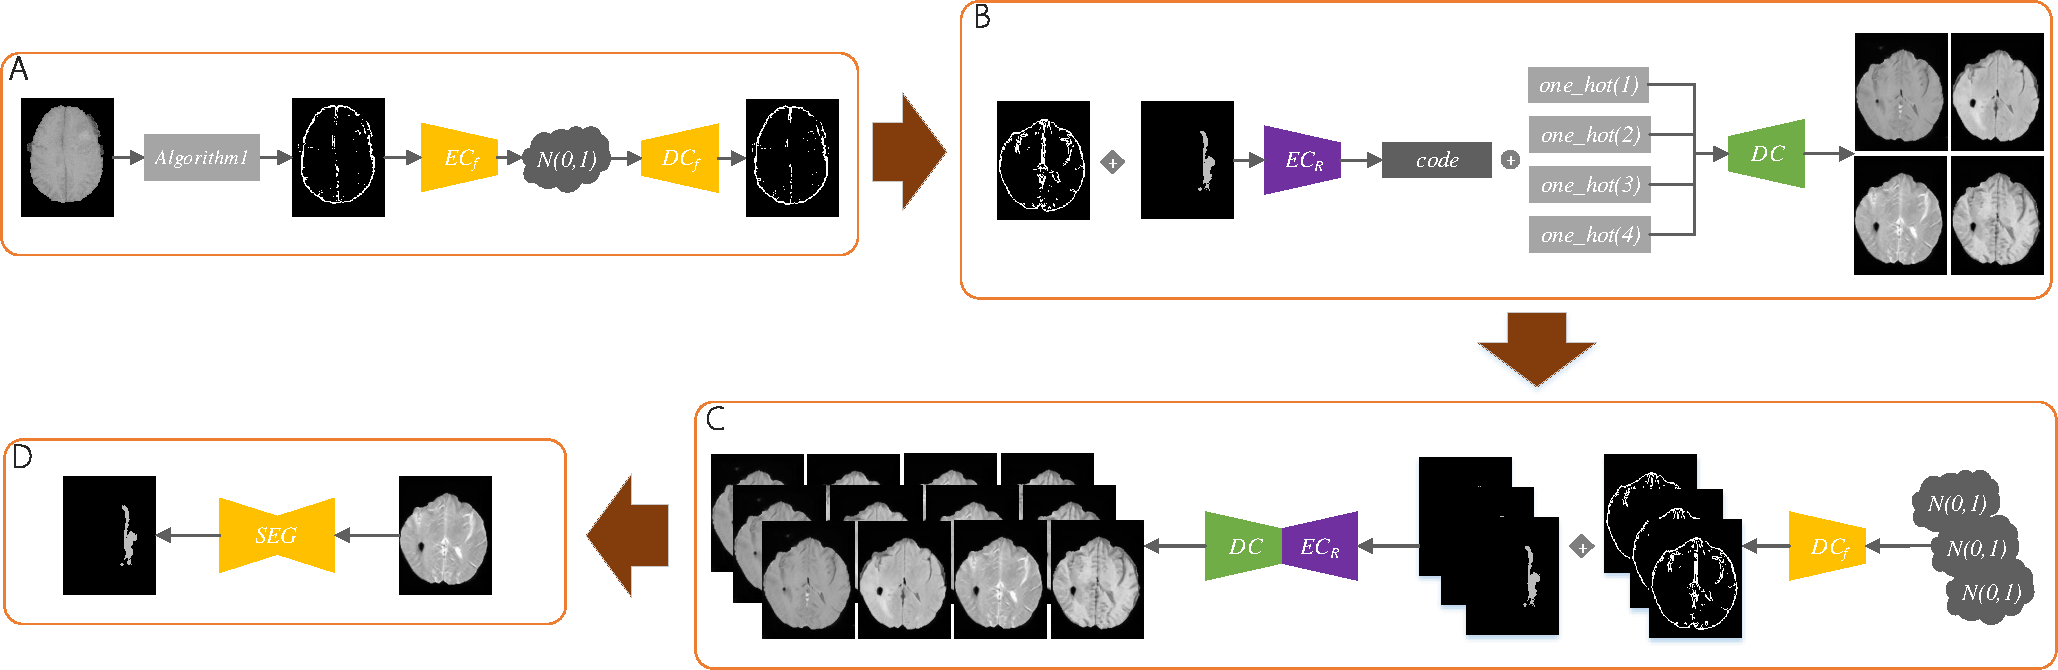
\includegraphics[width=0.98\linewidth]{figures/architecture}
	\caption{整体架构图.}
	\label{architecture}
\end{figure}

如图\ref{architecture}所示,我们的方案包括结构特征图提取和生成、多模态MRI生成、构建合成数据集、合成数据分割检测四个主要阶段。

结构特征图提取和生成阶段我们将获得一个结构特征图生成器,能从随机的正态分布矩阵生成结构特征图。该阶段我们训练的模型模包括一个结构特征图编码器、一个结构特征图解码器和一个结构特征图鉴别器。

多模态MRI生成阶段我们产出一个条件生成器,其以结构特征图为输入,能根据不同的独热条件向量生成不同模态的MRI,并且可在结构特征图上添加病灶标签使得生成的MRI具有对应的病灶信息。该阶段我们训练的模型模块包括一个结构特征与病灶标签融合图编码器、一组病灶标签分割组件、一个MRI编码器、一个MRI解码器、一个MRI鉴别器和一个MRI编码鉴别器。

在构建合成数据集阶段,我们使用前两个阶段产出的模型先从随机正态分布矩阵生成足量的结构特征图再随机添加病灶标签,最后生成配准的多模态MRI,构建出一个合成数据集。

在合成数据分割检测阶段,我们根据真实的数据为每个模态的MRI单独训练一个病灶分割网络,并在真实数据集中进行分割能力测试。此外,我们使用由不同比重的合成数据和真实数据构建的数据集来对病灶信息检测阶段中的病灶分割网络进行训练,训练充分后再在真实测试数据集上进行分割能力测试,对比各项测试结果,以验证合成数据在模型训练中的可用性。该阶段我们训练的模型包括每个模态的MRI的基于不同数据比重的病灶分割器。

\subsection{结构特征图提取方法}

直接从随机噪声通过生成对抗训练生成的医学影像通常训练困难且难以生成真实的结构信息。我们将医学影像中提供基本轮廓结构信息的图像称为其结构特征图,例如视网膜血管分布图可视为视网膜图像的结构特征图\cite{41costa2017towards}。结构特征图可以为医学影像的合成提供必要的指导信息,例如合成脑部MRI图像时一些研究从脑分割标签图获取基本的结构信息\cite{4shin2018medical}。然而,视网膜血管分布图和脑分割标签图等常用的结构特征图都需要额外的数据和训练才能实现从原图提取出结构特征图。为此,我们首先设计了一种直接从脑MRI提取结构特征图的方法,该方法具有运算快、无需训练、无需额外数据等优点。

在传统的数字图像处理方法中,Roberts算子\cite{87Roberts}、Prewitt算子\cite{88prewitt}、Sobel算子\cite{89Sobel}等是十分优秀的边缘检测算子,其中Sobel算子常用于脑部医学图像的处理,其卷积核参数和计算公式如图所示。我们探索出了从Sobel算子生成的边缘检测图中进一步提取结构特征的方法,如算法~\ref{alg:1}所示。
\begin{algorithm}
	\caption{Structural Feature Extraction}
	\label{alg:1}
	\begin{algorithmic}[1]
		\State 输入一张真实图像$n$,$beta$为元素阈值
		\State $f1 = reduce\_min(sobel(n))$
		\State $f2 = reduce\_max(sobel(n))$
		\State $f1 = mean(f1) - f1$
		\State $f2 = f2 - mean(f2)$
		\State $f1 = ones * (f1 > beta)$
		\State $f2 = ones * (f2 > beta)$
		\State $f = f1 + f2$
		\State $f = ones * (f > 0.)$
	\end{algorithmic}  
\end{algorithm}

简单来说,我们对一张真实图像用Sobel算子提取得到其横向和纵向的边缘检测图,对两张边缘检测图进行最大值规约和最小值规约得到两张新的边缘检测融合图,然后两张边缘检测融合图分别与各自的平均像素值求差,再对两张差值图根据设定像素阈值进行二值化处理,两张二值图求和后再进行完全的二值化,最后得到的就是我们需要的结构特征图。

\subsection{随机结构特征图的生成训练}

在生成结构特征图时,\cite{4shin2018medical}仍然需要真实的模态图作为输入来得到生成的结构特征图,这大大降低了生成数据的多样性,\cite{41costa2017towards}实现了一种从多维正态分布生成视网膜血管分布图的方法,在其基础上,我们设计了一种从随机噪声生成脑部结构特征图的方法,无需额外数据且具有更好的多样性。具体来说,我们结合了变分自编码器与生成对抗网络的特点设计了一种混合网络。首先,我们将从真实影像提取得到的结构特征图通过VAE的编码器编码为一个均值矩阵和一个方差矩阵,再与一个随机正态分布矩阵融合为一个潜在特征矩阵,并约束潜在特征矩阵服从多维正态分布,再用VAE的解码器实现从多维正态分布生成结构特征图。解码器通过特征图的自监督重建损失进行训练,对于潜在特征的约束方法,我们没有采用VAE的编码器损失,而是添加了一个鉴别器,鉴别器以正态分布矩阵为正样本、输入解码器的潜在特征矩阵为负样本进行学习,并为编码器提供对抗性损失,同时,我们通过L2正则损失指导均值矩阵的均值为0,标准差矩阵的均值为1。此外,我们用另一个鉴别器对真实的提取结构特征图与随机生成的结构特征图进行对抗学习,使生成的结构特征图越来越逼真。
\begin{figure}
	\centering
	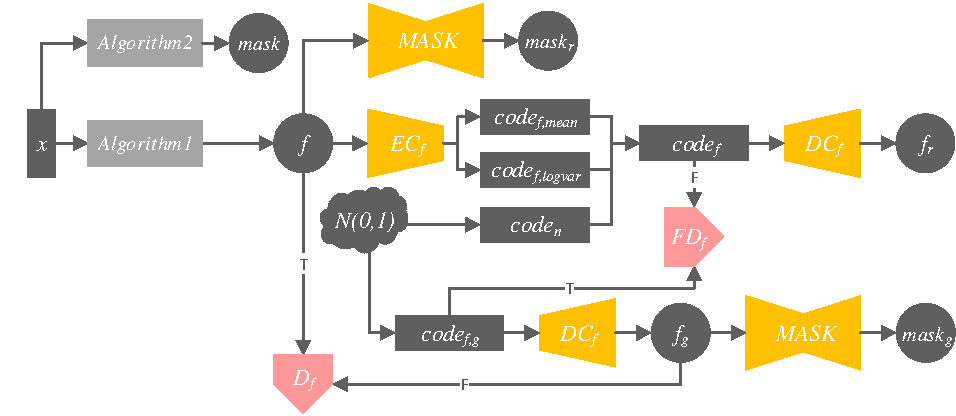
\includegraphics[width=0.98\linewidth]{figures/feature_train}
	\caption{随机结构特征图的生成训练.}
	\label{feature_train}
\end{figure}
如图~\ref{feature_train}所示,从标准正态分布解码得到随机结构特征图的具体处理过程如下:
\begin{itemize}
	\item 每次随机选择一个模态,从这个模态中获取一张图$M$,用结构特征提取方法得到结构特征图$f$,用掩模提取方法得到对应掩模$mask$;
	\item 用编码器$EC_f$对结构特征图$f$进行编码获得$code_{f,mean}$及$code_{f,logvar}$,从正态分布$\mathcal{N}(0,1^2)$的获取随机噪声$code_n$,由三个编码求得$code_f=code_{f,mean}+exp(0.5*code_{f,logvar})*code_n$;
	\item 用解码器$DC_f$对$code_f$解码得到重建的结构特征图$f_r$;
	\item 用掩模分割器$MASK$从$f$提取得到掩模$mask_r$;
	\item 随机生成符合正态分布$\mathcal{N}(0,1^2)$的矩阵$code_{f,g}$;
	\item 用解码器$DC_f$对$code_{f,g}$解码得到生成的随机结构特征图$f_g$;
	\item 用掩模分割器$MASK$对$f_g$提取得到掩模$mask_g$;
	\item 结构特征图鉴别器$D_f$分别对$f$和$f_g$进行鉴别,将前者鉴别为真,后者鉴别为假;
	\item 结构特征鉴别器$FD_f$分别对$code_f$和$code_{f,g}$进行鉴别,将前者鉴别为假,后者鉴别为真。
\end{itemize}

为了防止通过结构特征图生成的脑MRI像素区域超出结构特征图中脑轮廓线之外,我们还训练了一个从脑结构特征图获取脑部区域掩膜的生成器,该生成器与结构特征图的生成训练进行同步训练。训练时,从用于提取结构特征图的真实脑MRI中提取掩膜作为训练标签数据,掩膜的提取算法如算法2所示。
\begin{algorithm}
	\caption{Mask Extraction}
	\label{alg:2}
	\begin{algorithmic}[1]
		\State 输入一张真实图像$n$,$p$为扩充元素值
		\State $mask = 1.0 - ones * (n > 0.)$
		\State $shape = get\_shape(n)$
		\State $mask = resize(mask, size=[shape[1] + p, shape[2] + p])$
		\State $mask = crop\_padding(mask, crop\_length=p, crop\_width=p)$
	\end{algorithmic}  
\end{algorithm}
%\begin{quote}
%	\begin{scriptsize}\begin{verbatim}
%		算法2 掩模提取
%		1:输入一张真实图像n,p为扩充元素值
%		2:mask = 1.0 - ones * (n > 0.)
%		3:shape = get\_shape(n)
%		4:mask = resize(mask, size=[shape[1] + p, shape[2] + p])
%		5:mask = resize\_with\_crop\_or\_pad(mask, shape[1], shape[2])
%		\end{verbatim}\end{scriptsize}
%\end{quote}

在训练过程中,我们希望从随机正态分布矩阵解码出的结构特征图更逼真,所以通过鉴别器$D_f$对原图提取的结构特征与随机正态分布矩阵解码的结构特征进行对抗训练,此外,还通过特征鉴别器$FD_f$对真实结构特征图编码结果$code_f$与服从标准正态分布的矩阵$code_{f,g}$进行对抗训练,以此使得编码器$EC_f$能够将结构特征图F编码至标准正态分布。完整的损失函数如下,其中,$\omega_{i,j}$为各损失项的权重:
\begin{itemize}
	\item\textbf{结构特征对抗性损失} 
	这部分损失包括:使得结构特征图编码服从正态分布的对抗性损失,以及使得随机正态分布矩阵解码出结构特征图更逼真的对抗性损失

\begin{center}
	$loss_{FD_f}=\Vert{FD_f(code_{f,g})-1}\Vert_{2}^{2}+\Vert{FD_f(code_f)}\Vert_{2}^{2}$
\end{center}

\begin{center}
	$loss_{D_f}=\Vert{D_f(f)-1}\Vert_{2}^{2}+\Vert{D_f(f_g )}\Vert_{2}^{2}$
\end{center}

\begin{center}
	$loss_{G_f}=\Vert{FD_f(code_f)-1}\Vert_{2}^{2}+\Vert{D_f(f_g)-1}\Vert_{2}^{2}$
\end{center}

	\item \textbf{结构特征编码的监督损失} 
	这项损失使得结构特征图中间编码结果服从正态分布

\begin{center}
	$loss_{normal}=\Vert{mean(code_{f,mean})}\Vert_{2}^{2}+ \Vert{mean(exp(0.5*code_{f,logvar}))-1}\Vert_{2}^{2}$
\end{center}

	\item \textbf{结构特征图及掩模的自监督损失} 
	结构特征图和掩模两次重建融合后与原始结构特征图和掩模的两两自监督一致性损失

\begin{center}
	$loss_{sv}=\Vert{f-f_r}\Vert_{2}^{2}+\Vert{f_r*mask}\Vert_{2}^{2}$
\end{center}

	\item \textbf{Mask生成器损失}
	从$f$生成对应$mask$的Mask生成器损失
\begin{center}
	$loss_{mask}=\Vert{mask-mask_r }\Vert_{2}^{2}+\Vert{f*mask_r}\Vert_{2}^{2}+\Vert{f_r*mask_r}\Vert_{2}^{2}+\Vert{f_g*mask_g}\Vert_{2}^{2}$
\end{center}
\end{itemize}

\subsection{辅助的模态重建和模态转换训练}

在辅助的模态重建和模态转换训练中,我们用到了一套模态编码器、模态解码器和鉴别器,以及一组病灶标签生成组件,我们在真实的MRI上对这三个部件进行了下面同步的模态重建和模态转换训练,以约束三个部件在多模态MRI生成的训练中完成我们指定的学习任务。此外我们还通过一个特征鉴别器来对两个训练过程进行一致性指导。

\begin{figure}
	\centering
	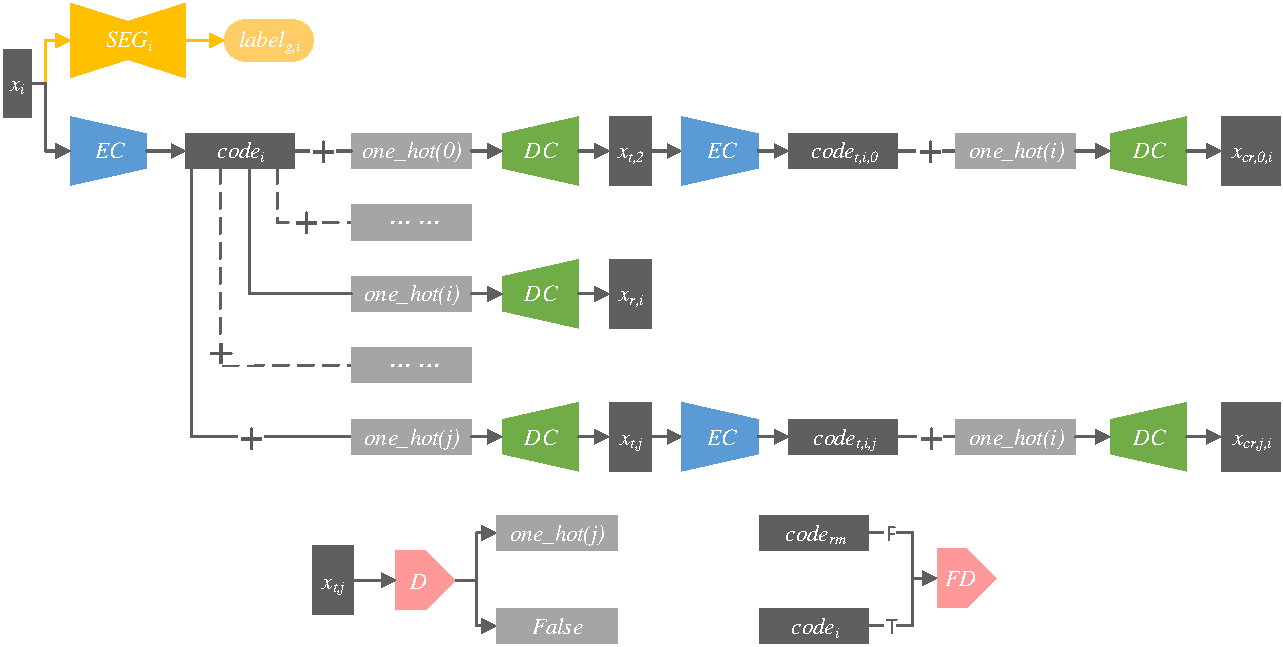
\includegraphics[width=0.98\linewidth]{figures/trans_train}
	\caption{辅助的模态重建和模态转换训练.}
	\label{trans_train}
\end{figure}

如图所示,模态转换和重建时,编码器将模态$i$的真实MRI$x_i$编码得到语义特征图$code_{x,i}$,然后我们将其与不同的条件向量连接,通过解码器解码出全部的模态。循环重建时,我们对所得到的转换图采用编码器全部进行再编码,将全部再编码得到的语义特征图均与模态$i$的条件向量进行连接,最后再用解码器全部解码得到循环重建的$x_{rc,i}$。模态重建的循环重建都是自监督训练。在上述过程中,我们以原始输入模态$x_i$对应的病灶标签$l_i$作为病灶还原训练的监督标签,对$x_i$用病灶标签生成组件得到$l_{r,i}$。

我们的鉴别器模块独立更新,其他模块通过一个优化器更新训练,损失项包括鉴别器提供的对抗性损失、模态重建自监督损失、模态循环重建自监督损失、模态循环重建一致性损失、语义一致性损失、病灶监督损失。详细损失如下,其中$x_{r,i})$表示模态$i$重建得到的MRI,$x_{j,t,i}$指由模态$j$转换生成的模态$i$的MRI,$d_{x,j,t,i}$和$c_{x,j,t,i}$分别为鉴别器对$x_{j,t,i}$的真假鉴别和类别鉴别结果,$x_{cr,j,i}$表示模态$i$转换为模态$j$再转换回模态$i$的MRI;$code_i$表示编$x_i$编码器编码后得到的语义特征图,$code_{i,t,j}$表示$x_i$转换生成的模态$j$的MRI再经过编码器编码后得到的语义特征图;$l_i$表示$x_i$的真实病灶标签,$l_{g,i}$表示$x_i$经过病灶标签生成组件生成的病灶标签:

\begin{itemize}
	\item 鉴别器损失
	
	\begin{center}
		$loss_{D,aided}=\sum\limits_{j=0,j\neq i}\sum\limits_{i=0}(\Vert{d_{x,j,t,i}}\Vert_{2}^{2}+\Vert{c_{x,j,t,i}-i}\Vert_{2}^{2})$
	\end{center}
	
	\item 对抗性损失和类别指导损失
	
	\begin{center}
		$loss_{G,aided}=\sum\limits_{j=0,j\neq i}\sum\limits_{i=0}(\Vert{d_{x,j,t,i}-1}\Vert_{2}^{2}+\Vert{c_{x,j,t,i}-i}\Vert_{2}^{2})$
	\end{center}
	
	\item 模态重建自监督损失
	
	\begin{center}
		$loss_{sv}=\sum\limits_{i=0}(\Vert{x_i-x_{r,i}}\Vert_{2}^{2})$
	\end{center}
	
	\item 模态循环重建自监督损失
	
	\begin{center}
		$loss_{cycle}=\sum\limits_{j=0,j\neq i}\sum\limits_{i=0}(\Vert{x_i-x_{cr,j,i}}\Vert_{2}^{2})$
	\end{center}
	
	\item 模态循环重建一致性损失
	
	\begin{center}
		$loss_{cycle,consistency}=\sum\limits_{k=0,k\neq j,k\neq i}\sum\limits_{j=0,j\neq i}\sum\limits_{i=0}(\Vert{x_{cr,j,i}-x_{cr,k,i}}\Vert_{2}^{2})$
	\end{center}
	
	\item 语义一致性损失
	
	\begin{center}
		$loss_{code,consistency}=\sum\limits_{j=0,j\neq i}\sum\limits_{i=0}(\Vert{code_i-code_{i,t,j}}\Vert_{2}^{2})$
	\end{center}
	
	\item 病灶监督损失
	
	\begin{center}
		$loss_{sv,l}=\sum\limits_{i=0}\Vert{l_i-l_{g,i}}\Vert_{2}^{2}$
	\end{center}
	
\end{itemize}

\subsection{结构特征图与分割标签图的融合}

我们已经可以得到从标准正态分布随机生成的结构特征图$f_g$,然后我们随机选择分割标签图$l$,将包含$n$个类别的分割标签图转为$n$个通道的独热矩阵$onehot_l$,每个通道对应一个分割类别,每个通道内的像素值为0或1,与对应类别分割位置相同的区域像素值为1其余部分为0,这样各个1像素区域与分割标签图中的各个分割区域是配准的。接下来,我们将$onehot_l$的每个通道与$f_g$按位求取加权和,得到一个新的融合了$f_g$和$l$信息的矩阵。

如果结构特征图$f'$是从随机MRI$m$中提取的,那么提取出的结构特征有可能包含肿瘤结构信息,会干扰与随机标签$l$中的肿瘤信息,影响融合后生成的图像,所以$f'$需要在与随机标签$l$融合前消除肿瘤信息,得到无肿瘤信息的结构特征图$f$,使生成图像的肿瘤信息只来源于标签$l$。我们通过$m$的分割标签$l_m$生成无边界扩充的分割掩膜$mask_{l,m}$,则$f=mask_{l,m}\times f'$。

由于随机选择的病灶的位置上可能出现在结构特征图的脑部轮廓之外,因此我们选取标签图时需要获取结构特征图的脑部区域掩膜$mask$,若$mask$与选取的$l$求积后为0,则说明肿瘤标签像素在$mask$的脑轮廓内部,可以采用,否则需要重新选取$l$。

\subsection{多模态MRI生成}
\begin{figure}
	\centering
	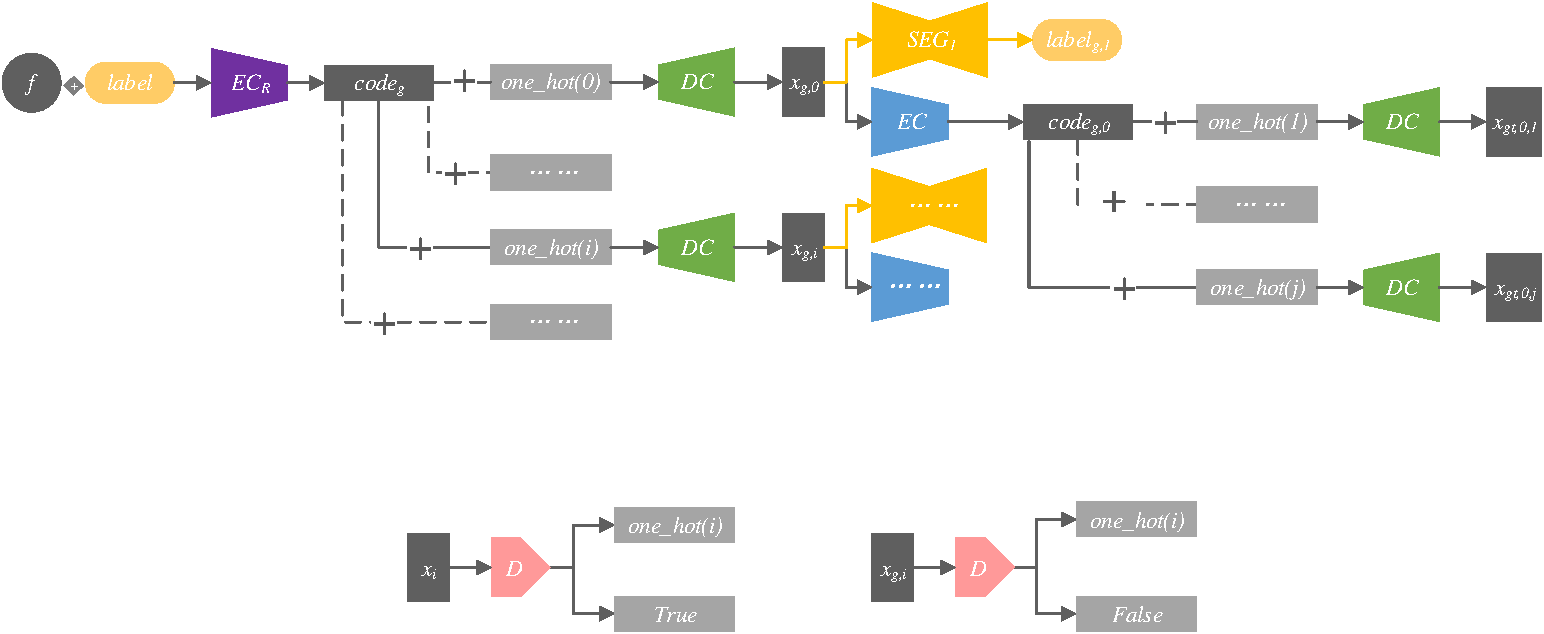
\includegraphics[width=0.98\linewidth]{figures/mm_mri_generate}
	\caption{多模态MRI生成.}
	\label{mm_mri_generate}
\end{figure}

结构特征图与分割标签图的信息融合图包含了目标部位的基本解剖结构信息和病灶信息,从该图生成多模态图比直接从随机噪声生成多模态图更易训练,生成的模态图更加合理和逼真。多模态MRI生成过程如图所示,首先,我们使用一个单独的编码器对信息融合图进行编码得到语义特征图,语义特征图与不同的条件向量堆叠后通过一个模态解码器解码,得到不同模态的合成图。我们通过一个模态鉴别器提供的对抗性损失和类别指导损失来使得生成的各个模态的合成图逼近于真实的MRI。各个模态的合成图再通过一个模态编码器得到模态语义特征图,然后这些语义特征图与不同的条件向量堆叠后通过模态解码器解码就实现了模态的转换,我们通过损失约束所有语义特征图的一致性,以及转换图的一致性,以此保证了生成的多模态影像互相配准。此外,我们使用一组病灶标签生成组件从各合成MRI中分割还原出肿瘤分割标签,确保生成的多模态影像根据输入病灶标签生成了对应的病灶内容。

我们的鉴别器模块独立更新,除只用于病灶标签生成组件中的模块外其他模块通过一个优化器更新训练,只用于病灶标签生成组件中的模块仅在辅助的转换和重建训练中采用真实数据训练更新,合成训练过程仅用于为生成模块提供语义指导损失。多模态MRI生成过程的具体损失函数如下,其中$d_{x,i}$和$c_{x,i}$为鉴别器$D(x_i)$的真假鉴别输出和类别鉴别输出,$d_{x,g,i}$,$c_{x,g,i}$为$D(x_{i,g})$的输出;$x_{g,i}$为模态$i$的合成图,$x_{g,j,t,i}$为模态$j$的合成图转换生成的模态$i$的转换图;$code_g$为输入信息编码后的语义特征图,$code_{x,g,i}$为$x_i$编码后的语义特征图;$l$为输入的标签图,$l_{x,g,i}$为$code_{x,g,i}$解码得到的重建标签图;$f$为输入的结构特征图,$f_{x,g,i}$为从$x_{g,i}$提取得到的结构特征图:

\begin{itemize}
	\item 使得随机正态分布矩阵解码出结构特征图更逼真的对抗性损失

\begin{center}
	$loss_{D}=\sum\limits_{i=0}(\Vert{d_{x,i}-1}\Vert_{2}^{2}+\Vert{d_{x,g,i}}\Vert_{2}^{2})$
\end{center}

\begin{center}
	$loss_{G}=\sum\limits_{i=0}(\Vert{d_{x,g,i}-1}\Vert_{2}^{2})$
\end{center}

	\item 模态类别指导损失

\begin{center}
	$loss_{D,class}=\sum\limits_{i=0}(\Vert{c_{x,i}-i}\Vert_{2}^{2}+\Vert{c_{x,g,i}-i}\Vert_{2}^{2})$
\end{center}

\begin{center}
	$loss_{G,class}=\sum\limits_{i=0}(\Vert{c_{x,g,i}-i}\Vert_{2}^{2})$
\end{center}

	\item 输入的结构特征图的重建自监督损失
	
\begin{center}
	$loss_{sv,f}=\sum\limits_{i=0}(\Vert{f-f_{x,g,i}}\Vert_{2}^{2})$
\end{center}

	\item 与输入的结构特征图融合后输入的肿瘤分割标签图的重建自监督损失
	
\begin{center}
	$loss_{sv,l}=\sum\limits_{i=0}(\Vert{l-l_{x,g,i}}\Vert_{2}^{2})$
\end{center}

	\item 生成的模态图进行转换得到的转换图与生成图的自监督损失

\begin{center}
	$loss_{trans}=\sum\limits_{j=0,j\neq i}\sum\limits_{i=0}(\Vert{x_{g,i}-x_{g,j,t,i}}\Vert_{2}^{2})$
\end{center}

	\item 自监督语义一致性损失
	
\begin{center}
	$loss_{trans,code}=\Vert{code_g-code_{x,g,i}}\Vert_{2}^{2}+\sum\limits_{j=0,j\neq i}\sum\limits_{i=0}(\Vert{code_{x,g,i}-code_{x,g,j}}\Vert_{2}^{2})$
\end{center}

\end{itemize}

\subsection{病灶标签生成组件设计方案}

我们设计了如下五组病灶标签生成组件。
\begin{itemize}
	\item \textbf{单分割器方案} 
	每个模态由一个共同的完整的分割器从合成的MRI还原得到各自的病灶标签。
	\item \textbf{单病灶编码器+多病灶解码器方案} 
	每个模态由一个采用共同的病灶编码器与每个模态的独立的病灶解码器组合得到的分割器,从合成的MRI还原得到各自的病灶标签。
	\item \textbf{多分割器方案} 
	每个模态由一个独立的完整的分割器从合成的MRI还原得到各自的病灶标签。
\end{itemize}
上述三种方案的损失函数与前文所述损失是一致的,各个模块均只使用辅助的模态重建和模态转换训练中的病灶监督损失进行训练,多模态MRI生成中的与输入的结构特征图融合后输入的肿瘤分割标签图的重建自监督损失只用于MRI生成组件的训练。

\subsection{构建合成数据集}
\label{make dataset}

如图所示,我们通过训练好的结构特征图解码器即可从随机生成的正太分布矩阵生成任意数量的结构特征图。然后,我们对原始的标签集进行了随机的缩放、旋转、平移、翻转等改变得到随机病灶标签集。我们再将随机生成的结构特征图和从随机病灶标签集中随机选择的病灶信息标签融合,同样地,我们借助生成的与结构特征图匹配的掩膜,可以筛选得到合适的随机病灶标签。最后,我们通过多模态生成模型即可从融合信息图中生成配准的多模态影像,选取的病灶信息标签就是生成的多模态影像的病灶标签。由此,我们可以从随机矩阵构建带有病灶标签的多模态配准影像数据集。
\begin{figure}
	\centering
	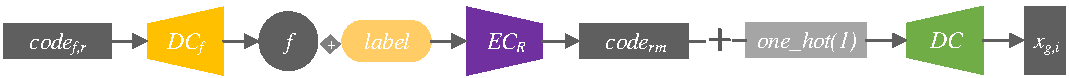
\includegraphics[width=0.98\linewidth]{figures/make_data}
	\caption{构建合成数据集.}
	\label{make_data}
\end{figure}

由于训练时去除肿瘤部分的结构的影响,合成的结构特征图中,存在一些质量较差的脑轮廓未闭合结构特征图,我们对此设计了一个结构特征图过滤算法。首先,我们使用生成器生成一张结构特征图和其对应的掩膜,我们先对结构特征图进行高斯模糊\cite{92wink2004denoising},再采用OpenCV[]提供的轮廓查找算法和填充算法获取高斯模糊图所有的闭合轮廓并进行填充,这样我们得到一个采用通常的算法的得到的掩膜,最后我们计算两张掩膜的均差(MAE)。若MAE低于我们设定的阈值则说明该结构特征图主要的脑部轮廓较为完整,该特征图可以使用;否则则说明该结构特征图主要的脑部轮廓有残缺,采用通常的算法得到的掩膜内部是空心的,与生成器生成的掩膜差异较大,因此,需要重新生成。算法表示如下:
\begin{algorithm}
	\caption{Structural feature map filtering}
	\label{alg:3}
	\begin{algorithmic}[1]
		\State \textbf{function} $GetMaskFromF(img)$
		\State \indent$contours = OpenCV.findContours(img)$
		\State \indent$img =OpenCV.drawContours(img,contours)$
		\State \indent\textbf{return} $img$
		\State \textbf{end function}
		\State
		\State $mae=0.05$
		\State \textbf{do} 
		\State \indent$f, m = Generator()$
		\State \indent$m'= GetMaskFromF(f)$
		\State \textbf{while} $MAE(m',m) <= mae$
	\end{algorithmic}  
\end{algorithm}
%\begin{quote}
%	\begin{scriptsize}\begin{verbatim}
%		算法3 结构特征图过滤
%		def get_mask_from_f(img):
%			contours = OpenCV.findContours(img)
%			img = OpenCV.drawContours(img,contours)
%			return img
%		
%		mae=0.05
%		while True:
%			f, m = Generator()
%			m_= get_mask_from_f(f)	
%			if MAE(m_,m) <= mae: break
%		\end{verbatim}\end{scriptsize}
%\end{quote}

从筛选出来的结构特征图和匹配的病灶标签得到的多模态MRI中,同样存在病灶信息生成情况较差的样本。此时,我们通过预先训练好的病灶分割网络对我们的合成MRI数据进行分割,然后将分割结果与输入的病灶标签进行骰子评分评估,只保留评分高于设定阈值(默认0.95)的样本。

经过多重筛选,我们得到最终的由随机结构特征图、配对掩膜、随机病灶分割标签、多模态MRI组成的合成数据集。我们要求该数据集使用在真实数据上训练得到的分割网络进行病灶分割时,得到的分割标签与数据集中的标签进行骰子分数评估,能取得0.99以上的分数。

\subsection{病灶分割}
\begin{figure}
	\centering
	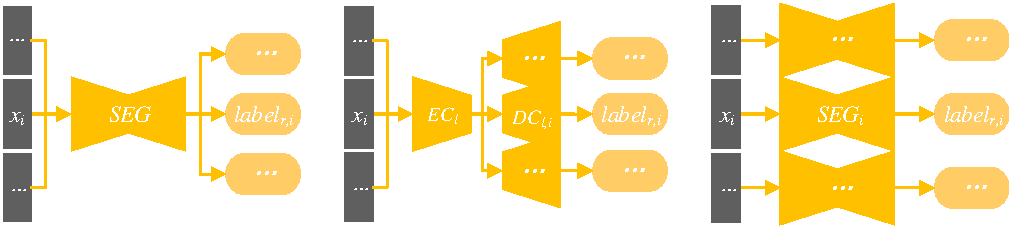
\includegraphics[width=0.98\linewidth]{figures/segmentation}
	\caption{病灶分割.}
	\label{segmentation}
\end{figure}

我们的病灶分割训练过程如图所示,为了验证合成数据中是否生成了与随机输入的病灶标签一致的病灶信息,我们用真实的数据为每个模态单独训练一个病灶分割网络,并在真实数据集中进行分割能力测试。然后使用训练好的分割器对合成数据集中的影像进行分割,将分割结果与输入的病灶标签比对评估,以此检验合成的影像中包含了预期的病灶信息。

此外,我们还采用由不同比重的合成数据和真实数据构建的数据集,来训练病灶分割网络,训练充分后再在真实测试数据集上进行分割能力测试,对比各项测试结果,以验证合成数据对分割训练的提升效果。

分割训练的损失函数如下,其中$l_{r,i}$表示$x_i$经过病灶分割器生成的病灶标签:

\begin{itemize}
	\item 病灶监督损失

	\begin{center}
		$loss_{l}=\sum\limits_{i=0}\Vert{l_i-l_{r,i}}\Vert_{2}^{2}$
	\end{center}
	
\end{itemize}

\section{实验}
\subsection{训练设置}

每项实验训练50个epoch;基础学习率分别为1e-4,无权重衰减;采用优亚当优化器,beta1取0.5;在输入层进行0.1的Dropout;Batch size为1;在生成器中使用均值滤波器的参数进行参数初始化,具体来说,对于一个卷积核尺寸为$[k,k,f]$的卷积层,我们采用random normal initializer设定该层卷积核的$k\times k\times f$个参数均设置为$1/(k\times k\times f)$, 偏置量为 0;在鉴别器中我们使用0均值和标准差为0.2的random normal initializer,偏置量为0。我们采用骰子分数\cite{95dice1945measures}和均方差(MSE)\cite{94prasad1990the}进行分割结果的评估,评估结果为2D图像的评估结果的均值,每项实验训练四次保留最佳结果。

\subsection{BRATS2015数据集}

我们采用了公开的BRATS2015\cite{91menze:hal-00935640}数据集进行实验,该数据集包含已配准的T1、T2、T1c、Flair四个模态,训练集每个模态有274张3D MRI,大小为155$\times$240$\times$240,同时配有274张相同尺寸的肿瘤分割标签。我们将样本按9:1划分训练集和测试集,取每张3D MRI第55-105间的50个slice构建2D的数据集。在数据预处理阶段,我们将每张图进行了标准化。

\subsection{BRATS合成数据集}

我们采用~\ref{make dataset}中的方法构建了一个配准的包含T1、T2、T1c、Flair四个模态的具有肿瘤标签的合成数据集。合成数据集样本的尺寸与BRATS2015数据集一致,但样本的多少可以根据实验需要进行任意数量的合成。

\subsection{BRATS增强数据集}

我们对原始的BRATS2015数据集进行了随机的缩放、旋转、平移、翻转等改变,得到增强数据。增强数据集样本的尺寸与BRATS2015数据集一致,但样本的多少可以根据实验需要进行任意数量的生产。

\subsection{病灶生成组件各方案对比实验}

我们使用在处理后的BRATS2015数据集的训练集对病灶分割网络进行了100个epoch的充分训练,然后我们在BRATS2015数据集的测试集和采用不同病灶生成组件方案的未经分割器筛选的的BRATS合成数据集上分别进行分割测试,除了测试数据来源的不同外,测试数据的样本量等其他条件完全相同。

\subsection{合成数据可用性验证实验}

如表所示,我们将真实的BRATS2015训练数据与BRATS合成数据进行了不同数量的混合,再用构建的混合数据集进行分割训练,最后再在真实的BRATS2015测试数据上进行模型的分割能力评估,所有实验都进行训练100个epoch的充分训练,除了训练数据源的不同外其他条件完全相同。同时,我们还进行了单独的合成数据的训练、真实数据与通常的数据增强数据的混合训练作为对比。我们设定了随机混合、先真后假、先假后真三种数据混合方式。

\section{结果}
\subsection{实验量化结果}

\subsubsection{病灶检测实验结果}
\begin{table}[t]
	\caption{病灶检测实验结果.}\smallskip
	\centering
	\resizebox{.95\columnwidth}{!}{		
		\smallskip\begin{tabular}{l|l|l|l}			
			synthetic method&test data type &MSE   &Dice Score \\			
			-&real 		   				&0.014 &0.961 \\					
			1SEG&synthetic     			&0.053 &0.741 \\			
			1ECL+4DCL&synthetic     	&0.055 &0.808 \\		
			4SEG&synthetic     			&0.043 &0.838 \\			
		\end{tabular}
		
	}	
	\label{label_test}	
\end{table}

如表~\ref{label_test}所示,我们在BRATS2015训练数据经过100个epoch的充分训练后,在真实的测试数据集上,分割测试结果达到了0.014的MSE和0.961的SSIM\cite{93wang2004image}。之后我们使用这个表现优秀的分割网络对我们未经过滤的合成数据进行分割测试,在与真实测试数据集相同数据量的合成数据集上,不同病灶标签生成组件设计方案都取得了较好的分割结果,其中一个模态一个分割器的方案取得了最好的结果,Dice Score也达到了0.838。

\subsubsection{合成数据可用性验证实验结果}
\begin{table}[t]
	\caption{合成数据可用性验证实验结果.}\smallskip
	\centering
	\resizebox{.95\columnwidth}{!}{
		\smallskip\begin{tabular}{l|l|l|l|l|l|l}
			序号 & 真实量 & 合成量 & 增强量  & 混合方式  & MSE &Dice Score\\
			1& 15070 & 0  &0 &无混合 &0.033 &0.954 \\
			31& 15070$\times$ 0.5 & 0  &0 &无混合 & & \\
			2& 0 & 15070  &0 &无混合 & & \\
			
			3& 0 & 15070$\times$ 2  &0 &随机混合 & & \\
			4& 0 & 15070$\times$ 3  &0 &随机混合 & & \\
			%5& 0 & 15070$\times$ 4  &0 &随机混合 & & \\
			%6& 0 & 15070$\times$ 5  &0 &随机混合 & & \\
			
			7& 15070$\times$ 0.1 & 15070  &0 &先假后真 & & \\
			8& 15070$\times$ 0.1 & 15070$\times$ 2  &0 &先假后真 & & \\
			9& 15070$\times$ 0.1 & 15070$\times$ 3  &0 &先假后真 & & \\
			%10& 15070$\times$ 0.1 & 15070$\times$ 4  &0 &先假后真 & & \\
			%11& 15070$\times$ 0.1 & 15070$\times$ 5  &0 &先假后真 & & \\
			
			12& 15070$\times$ 0.5 & 15070$\times$ 0.5 &0  &随机混合 & & \\
			13& 15070$\times$ 0.2 & 15070$\times$ 0.8 &0  &随机混合 & & \\
			14& 15070$\times$ 0.8 & 15070$\times$ 0.2 &0  &随机混合 & & \\
			32& 15070 & 15070$\times$ 0.2 &0  &随机混合 & & \\
			33& 15070 & 15070$\times$ 0.5 &0  &随机混合 & & \\
			34& 15070 & 15070$\times$ 0.8 &0  &随机混合 & & \\
			15& 15070 & 15070 &0  &随机混合 & & \\
			16& 15070 & 15070 &0  &先真后假 & & \\
			17& 15070 & 15070 &0  &先假后真 & & \\
			
			18& 15070 & 15070$\times$ 2  &0 &随机混合 & & \\
			19& 15070 & 15070$\times$ 3  &0 &随机混合 & & \\
			%20& 15070 & 15070$\times$ 4  &0 &随机混合 & & \\
			%21& 15070 & 15070$\times$ 5  &0 &随机混合 & & \\
			
			35& 15070 &0 & 15070$\times$ 0.2   &随机混合 & & \\
			36& 15070 &0 & 15070$\times$ 0.5   &随机混合 & & \\
			37& 15070 &0 & 15070$\times$ 0.8   &随机混合 & & \\
			22& 15070 &0 & 15070 &随机混合 & & \\
			23& 15070 &0 & 15070$\times$ 2 &随机混合 & & \\
			24& 15070 &0 & 15070$\times$ 3 &随机混合 & & \\
			%25& 15070 &0 & 15070$\times$ 4 &随机混合 & & \\
			%26& 15070 &0 & 15070$\times$ 5 &随机混合 & & \\
		\end{tabular}
	}
	\label{use_test}
\end{table}
如表~\ref{use_test}所示,我们在不同的成分和数量的数据集上都经过训练后再在真实测试集上评估,得到了表中的结果。实验1在BRATS2015训练数据经过100个epoch的充分训练后,在真实的测试数据集上,分割测试结果达到了0.033的MSE和0.954的SSIM。从表中实验2-4单独使用合成数据训练的结果看,与真实数据的训练结果有一定差距,说明我们的合成数据尚不能完全替代真实数据充当训练集。实验7-9结果表明使用大量合成数据进行预训练,再在少量真实数据上微调能达到和实验1全使用真实数据训练十分接近的结果。实验12-14一定比例的真实数据与合成数据随机混合,能达到和真实数据训练差不多的效果,比例相近时效果与实验1相差不大,合成数据比例偏高时,结果比实验1略低,合成数据比例偏低时,能提供模型的泛化能力,取得高于实验1的结果。实验15-17等比例混合真实数据与合成数据,随机混合时合成数据用作数据增强,效果比真实数据训练效果好,说明合成数据起到数据增强的作用,能有效提升训练效果;先训练真实数据再用合成数据进行补充训练,结果较差,与完全使用合成数据训练效果差不多;先使用合成数据进行与训练,再使用真实数据进行训练,能取得非常好的结果。实验15,32-34,18-19按多种比例混合真实数据与合成数据,开始时(实验33-34,15)随着合成数据的增加能提升训练效果,但随着合成数据比例继续增大,训练效果会下降。最后实验35-37,22-24是使用传统数据增强方法进行数据增强,实验结果表明合成数据比传统数据增强的训练效果更好。
但在真实数据充当训练集的基础上,可以使用合成数据集作为增强数据来提高模型泛化能力,数据最好的组合使用方式是随机混合使用。我们也注意到,合成数据也并不是越多越好的,当合成数据所占比重过大时,为降低真实数据的影响力。在我们的实验中,采用【】倍的合成数据与真实数据进行随机混合取得了最好的提升效果,相比完全的真实数据,分割测试结果提升了【\%】的MSE和【\%】的SSIM,远远大于通常的数据增强的提升幅度。与\cite{4shin2018medical}的结论一致,我们的合成数据也可用于预训练,然后再使用少量真实数据微调,最后能得到和完全真实数据训练相竞争的结果。

\subsection{合成数据可视化}

上述各项实验的一些生成结果如图~\ref{generated_f}~\ref{generated_mri}~\ref{label_from_diff_test}~\ref{label_from_diff_train}所示,从图中我们能更直观的取得结论。
\begin{figure}
	\centering
	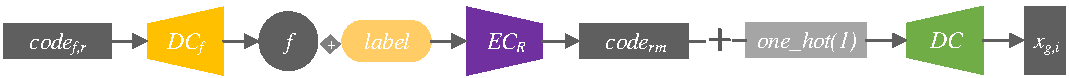
\includegraphics[width=0.98\linewidth]{figures/make_data}
	\caption{合成的结构特征图机器掩膜.}
	\label{generated_f}
\end{figure}

\begin{figure}
	\centering
	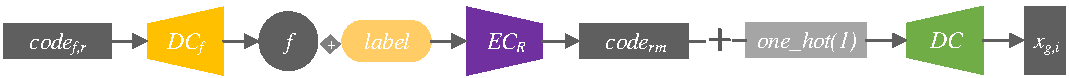
\includegraphics[width=0.98\linewidth]{figures/make_data}
	\caption{合成的多模态MRI.}
	\label{generated_mri}
\end{figure}

\begin{figure}
	\centering
	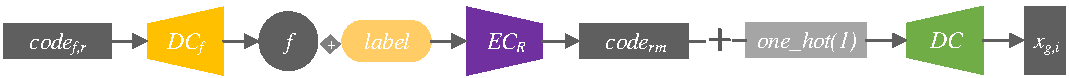
\includegraphics[width=0.98\linewidth]{figures/make_data}
	\caption{使用真实训练数据的分割模型在不同测试集上的分割示例.}
	\label{label_from_diff_test}
\end{figure}

\begin{figure}
	\centering
	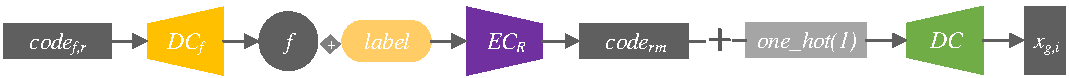
\includegraphics[width=0.98\linewidth]{figures/make_data}
	\caption{使用不同训练数据的分割模型在真实测试集上的分割示例.}
	\label{label_from_diff_train}
\end{figure}

\section{结论与未来工作}

我们基于条件生成对抗网络,通过无监督的训练,实现了能在已有单模态数据时可扩展出多模态影像数据并保留原模态的病灶信息,同时可从随机噪声生成配准的多模态医学影像并可自由添加病灶信息。我们通过病灶分割实验验证了合成的医学影像可以用于医学影像智能处理任务的预训练或者补充训练来提高模型的泛化能力。具体来说,我们的贡献包括以下几点:
\begin{itemize}
	\item 结构特征图提取方法。我们从医学影像直接提取解剖结构信息,无须训练,无需额外数据;
	\item 随机结构特征图生成方法。我们实现了从多维正态分布采样生成结构特征图,使结构特征图能便捷地大量生成并使最后合成的影像具有良好的多样性;
	\item 模态转换方法。我们实现了多模态脑MRI之间的互转,使单模态数据可转换生成多模态影像数据并保留原模态的病灶信息;
	\item 基于结构特征图生成多模态图方法。我们从真实影像提取的结构特征图及随机选择的标签生成带病灶标签的配准的多模态影像;
	\item 构建带标签的多模态配准数据集方法。我们组合使用随机结构特征图生成方法和基于结构特征图生成多模态图方法,实现了从多维正态分布随机生成结构特征图,结合随机选择的标签生成带标签的配准的多模态MRI数据;
	\item 合成数据可用性测试方法。我们将合成数据与真实数据数据集进行不同比重的混合,通过病灶分割网络验证了合成数据在分割训练中的提升效果。
\end{itemize}

未来,我们将进一步在CT、PET等不同模态和其他部位中对我们的方法进行改进,并将进一步简化训练过程和提升合成质量。	

\section{ Acknowledgments}

感谢NSCCGZ提供的计算支持。

\bibliographystyle{unsrt}

\bibliography{refer}

\end{document}
